\section{Formalization of Untriggered Statecharts}
\label{sec:utsc}
In this section, we formalise the syntactic elements and semantics of untriggered statecharts.
This  includes finding sufficient conditions for well-defined untriggered statecharts to guarantee consistent semantic behaviour of such models.
The main ideas for our formalisation are 
(1) to use the \EventB \emph{contexts} to capture the \emph{syntactic elements} of the model with axioms ensuring that the model is well-defined (Section~\ref{sec:utsc-syntax}), and 
(2) to use the \EventB \emph{machines} to capture the \emph{semantics} of the models (Section~\ref{sec:utsc-semantics}).

\subsection{Formalisation of the Untriggered Statechart Syntactic Elements}
\label{sec:utsc-syntax}
As the syntactic elements of untriggered statecharts are fairly complex, we develop them gradually, together with their well-definedness conditions,  using \EventB context extension in the following steps.
\begin{enumerate}
    \item Model the tree-structure of the states
    \item Model the parallel regions
    \item Model the transformations between states
\end{enumerate}

\subsubsection{Tree-structure States} The structure of the states of a statechart is represented by  the following constants; |states| (the set of all states), |root| (the implicit root state), |container| (the relationship between a child state and its parent container), |leaves| (the set of leaf states). 
These constants satisfy an axiom stating that they form a tree-shaped structure (here |↦| is the notation for specifying tuples).
\begin{center}
    |states ↦ root ↦ container ↦ leaves ∈ Tree|
\end{center}
Where, |Tree| is a constant, defined using transitive closure, that formalises the definition of tree-shaped structures. 
An important derived property of a tree-shaped structured (proved as a theorem) is needed to allow us to prove properties by induction.
\begin{theorem}[Tree induction from root]
\label{thm:tree-induction}
    Consider a property |P|. If 
    \begin{enumerate}
        \item The |root| satisfies |P|, and
        \item for every non-root state |s|, if the container of |s|, i.e., |container(s)|, satisfies |P|, then |s| also satisfies |P|,
    \end{enumerate}
    then every state in the tree satisfies |P|.
\end{theorem}
%\begin{figure}
%    \centering
%    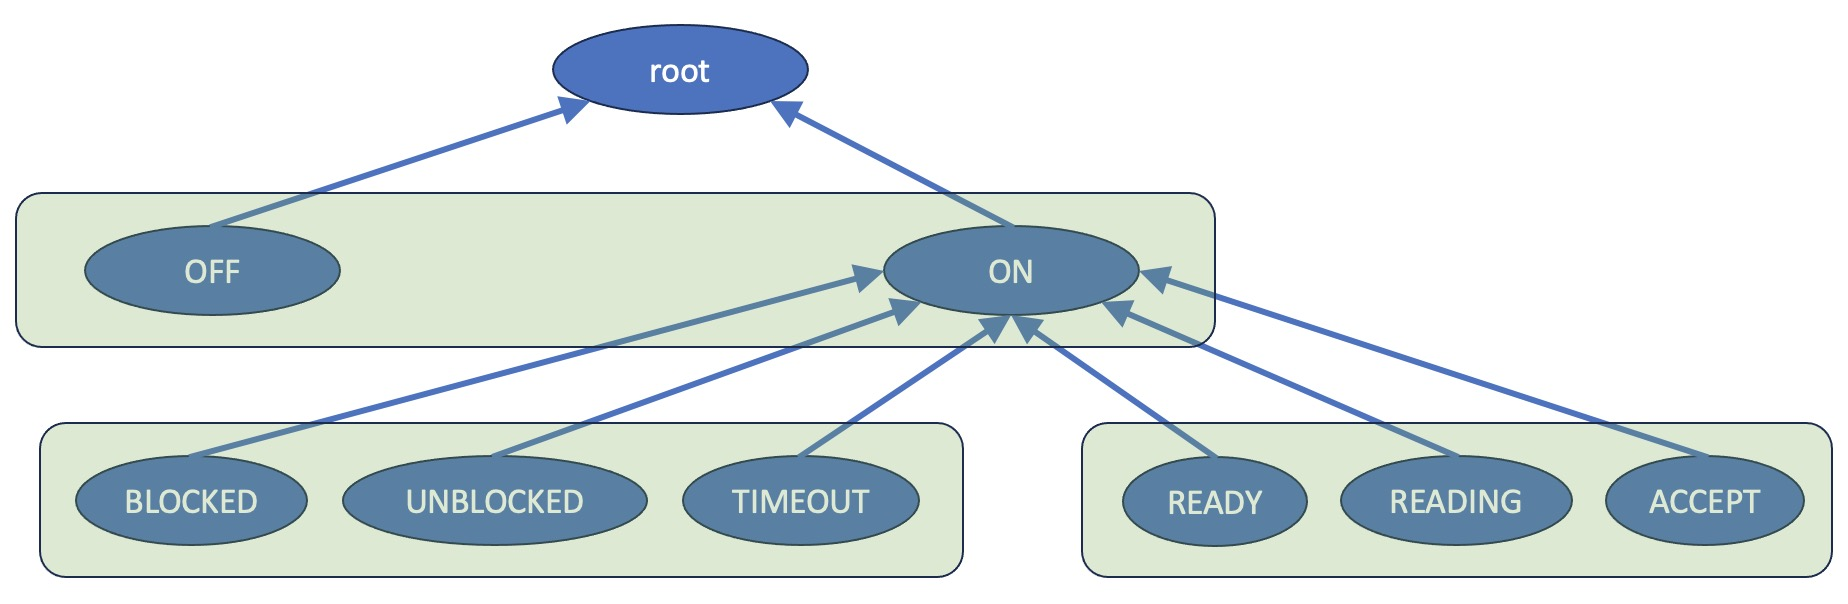
\includegraphics[width=0.8\textwidth]{figures/TreeShapedStates}
%    \caption{The states and regions structure for the turnstile example}
%    \label{fig:turnstile-tree-shaped}
%\end{figure}

\begin{example}[Turnstile Example. Tree-shaped Structure States]
%    The tree-shaped structure of states in the turnstile example can be seen in Figure~\ref{fig:turnstile-tree-shaped}.
    Formally, we have the following definitions.   
\begin{EventBcode}
// All states of the turnstile examples
partition(states, {root}, {OFF}, {ON}, {BLOCKED}, {UNBLOCKED}, {TIMEOUT},
    {READY}, {READING}, {ACCEPT})
// The container relationship between states
container = {OFF ↦ root, ON ↦ root, BLOCKED ↦ ON, UNBLOCKED ↦ ON,
    TIMEOUT ↦ ON, READY ↦ ON, READING ↦ ON, ACCEPT ↦ ON}
// leaf states
leaves = {BLOCKED, UNBLOCKED, TIMEOUT, READY, READING, ACCEPT, OFF}
\end{EventBcode}

The |partition| operator defines an enumerated set, |states|, where all the elements are explicitly given.
\end{example}

\subsubsection{Regions} Untriggered statecharts support the parallel composition of two or more nested statechart regions. 
That is a single state of a statechart may represent several sub components and associate with each component a corresponding region.
In the turnsile example, the container state \emph{ON} has two regions \emph{GATE} and \emph{CARD\_READER}. 
We formalise the notion of regions as partitions of the set of non-root states by using the following axioms to constrain the constant |regions|.

\begin{axiom}[Regions are subsets of states]
\label{axm:@region_type}
Each region is a subset of the statechart's states. (Here |ℙ| is the notation for powerset.)
    \begin{center}
        \EventBInline{@region_type: regions ⊆ ℙ(states)}
    \end{center}
\end{axiom}
\begin{axiom}[Regions are disjoint]
\label{axm:@region_disjoint}
Every pair of distinct regions does not share any states.
    \begin{center}
        \EventBInline{@region_disjoint: !r1, r2 · r1 ∈ regions ∧ r2 ∈ regions ∧ r1 ≠ r2 ⇒ r1 ∩ r2 = ∅}
    \end{center}    
\end{axiom}
\begin{axiom}[Regions cover non-root states]
\label{axm:@region_complete}
Every non-root state belongs to a region.
    \begin{center}
        \EventBInline{@region_complete: union(regions) = states \ \{root\}}
    \end{center}
\end{axiom}
\begin{axiom}[Region has a unique container]
\label{axm:@region_same_parent}
Every region has a unique container state. Here |container[region]| is the image of the relation |container| applying to |region|.
    \begin{center}
        \EventBInline{@region_same_parent: ! region · region ∈ regions ⇒}\\
        \EventBInline{ (∃parent · container[region] = \{parent\})}
    \end{center}
\end{axiom}

\begin{example}[Turnstile Example. Regions]
   % The parallel regions for the turnstile example can be seen in Figure~\ref{fig:turnstile-tree-shaped}.
    Formally, we have three regions as follows.
\begin{EventBcode}
regions = { {ON, OFF}, // TURNSTILE region
	{BLOCKED, UNBLOCKED, TIMEOUT}, // GATE region
	{READY, READING, ACCEPT}	// CARD_READER region
}
\end{EventBcode}
Note that states |ON| and |OFF| implicitly form a region without any sibling parallel region.
\end{example}

\subsubsection{Transformations} Unlike the common definitions of transitions, which map a source state to a target state, we define |transformations|, which give an hierarchical view of the set of all simultaneously enabled transitions of the system, from one \emph{enabling} state configuration to the next configuration. 
There are different types of transformation including 
\emph{forking} (starting from a state and ending in one or more states in different parallel regions), 
\emph{joining} (starting from two or more states in different parallel regions and ending in a state), \emph{parallel} (updating parallel regions at the same time), 
and any combination of these types. 
To model all transformation types, we formalise each transformation by three sets of states.
\begin{itemize}
\item |enabling|: A transformation is enabled (i.e., can be executed)
  if its (non-empty) set of enabling states are active.
  
\item |exiting|: The (possibly empty) set of states that the transformation
  will exit upon execution.
  
\item |entering|: The (possibly empty) set of states the transformation will enter upon
  execution.
\end{itemize}
Formally, these notions are formalised as constants as follows.
\begin{EventBcode}
enabling ∈ transformations → ℙ1(states)
exiting ∈ transformations → ℙ(states)
entering ∈ transformations → ℙ(states)
\end{EventBcode}

\begin{example}[Turnstile Example. Transformation]
We give the enabling, exiting, entering and active states of the following example transformations.
\begin{itemize}
    \item Consider the transformation from the |BLOCKED| state to the |UNBLOCKED| state, we call this |BLOCKED_2_UNBLOCKED|. We have
\begin{EventBcode}
enabling(BLOCKED_2_UNBLOCKED) = {BLOCKED}
exiting(BLOCKED_2_UNBLOCKED) = {BLOCKED}
entering(BLOCKED_2_UNBLOCKED) = {UNBLOCKED}
\end{EventBcode}

    \item Consider the transformation from the |OFF| state to the |ON|
state, we call this |OFF_2_ON|. Notice that the transformation will take into account also the transition from the initial states within the two sub-statecharts (regions). As a result, we have
\begin{EventBcode}
enabling(OFF_2_ON) = {OFF}
exiting(OFF_2_ON) = {OFF}
entering(OFF_2_ON) = {ON, BLOCKED, READY}
\end{EventBcode}

    \item Consider the transformation from the |ON| state to the |OFF|
state, we call this |ON_2_OFF|. Notice that the transformation will take into account the non-deterministic exit from the two sub-statecharts (regions). As a result, we have
\begin{EventBcode}
enabling(ON_2_OFF) = {ON}
exiting(ON_2_OFF) = {ON, BLOCKED, UNBLOCKED, TIMEOUT, READY, READING, ACCEPT}
entering(ON_2_OFF) = {OFF}
\end{EventBcode}
\end{itemize}
\end{example}

There are several additional constraints (well-definedness conditions) relating the enabling, exiting, and entering states for a transformation. We identified some of the constraints directly. For instance, the following axioms related to |exiting| states.
\begin{axiom}[Exiting a contained region]
\label{axm:@exiting-contained_region}
If the container of a region is an exiting state, there must be an exiting state within that region. Here |container[r]|, is the image of the relation container applying to region |r|.
\begin{EventBcode}
@exiting-contained_region:
    ∀trf, s, r · trf ∈ transformations ∧ s ∈ exiting(trf) ∧ r ∈ regions ∧ container[r] = {s}
        ⇒ exiting(trf) ∩ r ≠ ∅
\end{EventBcode}
\end{axiom}

\begin{axiom}[Exiting one or all states in a region]
\label{axm:@exiting-either_one_or_all_in_a_region}
If a region |r| has an exiting state |s| then either |s| is the unique exiting state or all the states in |r| are exiting states.
\begin{EventBcode}
@exiting-either_one_or_all_in_a_region: 
    ∀trf, s, r · trf ∈ transformations ∧ s ∈ exiting(trf) ∧ r ∈ regions ∧ s ∈ r
        ⇒ exiting(trf) ∩ r = {s} ∨ r ⊆ exiting(trf)
\end{EventBcode}
\end{axiom}

The following axioms linking |exiting| and |enabling| states was ``discovered'' during the proof of the invariant preservation proof obligations (see Theorem~\ref{po:transformation/active_container/INV}).
\begin{axiom}[Exiting a unique enabling state in a region]
\label{axm:@exiting-unique_enabling_state_in_a_region}
Given a region |r| and an exiting state |s| in |r|, if |r| has states other than |s|, |s| must be the unique enabling state in |r|.
\begin{EventBcode}
@exiting-unique_enabling_state_in_a_region:
    ∀trf, s, r · trf ∈ transformations ∧ r ∈ regions ∧ exiting(trf) ∩ r = {s} ∧ r ≠ {s}
        ⇒ enabling(trf) ∩ r = {s}
\end{EventBcode}
\end{axiom}
\begin{axiom}[Enabling state is the unique exiting state]
\label{axm:@enabling-unique_exiting_state_in_a_region}
Given a region |r| with some exiting state, an enabling state |s| in |r|, |s| must the unique exiting state in |r|.
\begin{EventBcode}
@enabling-unique_exiting_state_in_a_region:
    ∀trf, s, r · trf ∈ transformations ∧ s ∈ enabling(trf) ∧
    exiting(trf) ∩ r ≠ ∅ ∧ r ∈ regions ∧ s ∈ r ⇒ exiting(trf) ∩ r = {s}
\end{EventBcode}
\end{axiom}

The following axiom relates |entering| with |enabling| and |exiting| states. It is also discovered during the proof of the invariant preservation proof obligations (see Theorem~\ref{po:transformation/active_container/INV}).
\begin{axiom}[Transformation stays within a state]
\label{axm:@entering-stay_within_state}
If a transformation enters a region |r| but not the container of |r| (called |c|), then |c| is not an exiting state and there is an enabling state which is a descendant of |c|. Here, |cl(container)| denote the transitive closure of |container| relationship, hence the inverse of that (i.e., |cl(container)∼| is the descendant relationship between states.
\begin{EventBcode}
@entering-stay_within_state:
    ∀trf, r, c · trf ∈ transformations ∧ r ∈ regions ∧ container[r] = {c} ∧
    entering(trf) ∩ r ≠ ∅ ∧ entering(trf) ∩ container[r] = ∅
        ⇒ enabling(trf) ∩ cl(container)∼[{c}] ≠ ∅ ∧ c ∉ exiting(trf) 
\end{EventBcode}
\end{axiom}


\subsection{Formalisation of the Untriggered Statechart Semantics}
\label{sec:utsc-semantics}

Given an untriggered statechart (characterized by the tree-shape structured states, the regions, and the transformation), the semantics of the statechart is characterized by the set of active states during its execution. For instance, consider the turnstile example in Figure~\ref{fig:turnstile}, initially, the turnstile has one active state, namely |OFF|, i.e., the set of active states is |{OFF}|
\begin{itemize}
    \item A transformation |OFF_2_ON| (from |OFF| to |ON|) will change the set of active states to |{ON, BLOCKED, READY}|.
    \item A transformation |BLOCKED_2_UNBLOCKED| will change the set of active states to |{ON, UNBLOCKED, READY}|.
    \item A transformation |ON_2_OFF| changes the set of active states to |{OFF}|.
\end{itemize}

We can now formalize the semantics of the untriggered statechart in a machine using a single variable |active| satisfying |active ⊆ states|. 
The system's functionality is encoded through one event called |transformation| that captures how the design transitions from one configuration to the next. 
Essentially variable |active| provides a discrete characterization of the information and event |transformation| represents the operation of the system under analysis. 
\begin{EventBcode}
event transformation
any trf where
	@typeof-trf: trf ∈ transformations
	@active-enabling: enabling(trf) ⊆ active
then
	@update-active: active ≔ (active ∖ exiting(trf)) ∪ entering(trf)
end
\end{EventBcode}
Guard |@active-enabling| ensures that the chosen transformation |trf| is enabled and action |@update-active| first removes the |trf|'s exiting states then adds |trf|'s entering states.  Notice that this action also allows a transformation to exit a state and re-enter that state.

An important aspect for the semantics of statecharts is that it can only transform amongst valid configurations.  For example, we want to ensure that the turnstile statechart is never in the configuration where both |ON| and |OFF| states are active or in a state where |BLOCKED| is active, but |ON| is not active. The following constraints on |active| specify the valid configuration for a statechart, which we encode as 4 invariants for the machine.
\begin{invariant}[Container active]
\label{inv:container_active}
If a non-root state is active then its container is also active.
\begin{center}
\EventBInline{@container_active: ∀ s · s ∈ active ∖ {root} ⇒ container(s) ∈ active}
\end{center}
\end{invariant}
\begin{invariant}[Content active]
\label{inv:content_active}
If a container state is active then one of its sub-state must be active.
\begin{center}
\EventBInline{@content_active: ∀ s · s ∈ ran(container) ∧ s ∈ active ⇒}\\
\EventBInline{container∼[\{s\}] ∩ active ≠ ∅}
\end{center}
where |ran(container)| is the range of the container relation
\end{invariant}
\begin{invariant}[Unique active state within a region]
\label{inv:active-region-unique}
There can be at most one active state in a region.
\begin{center}
\EventBInline{@active-region-unique: ∀r, s · r ∈ regions ∧ s ∈ r ∩ active ⇒ r ∩ active ⊆ \{s\}}
\end{center}
\end{invariant}
\begin{invariant}[Parallel regions are inactive/active at the same time]
\label{inv:active-region-parallel}
All parallel regions are inactive (hence active) at the same time.
\begin{center}
\EventBInline{@active-region-parallel: ∀r1, r2 · r1 ∈ regions ∧ r2 ∈ regions ∧} \\
\EventBInline{container[r1] = container[r2] ∧ r1 ∩ active = ∅ ⇒ r2 ∩ active = ∅}
\end{center}
\end{invariant}
As a consequence of Invariant~\ref{inv:container_active}, we can prove the following machine theorem. Note that all proofs related to this work were discharged semi-automatically within Rodin using the Proving Perspective. We present the general structure of a selected subset of these proofs.
\begin{theorem}[Ancestors active]
\label{thm:@ancestor_active}
If a state |s| is active then all ancestors of |s| are also active.
\begin{center}
\EventBInline{@ancestor_active:	∀ s · s ∈ active ⇒ cl(container)[{s}] ⊆ active}
\end{center}
\end{theorem}
\begin{proof}
The proof of the theorem relying on Invariant~\ref{inv:container_active} and the inductive nature of transitive closure. We omit the details here.
\end{proof}

We have to prove that event |transformation| maintains the  invariants relying on the well-definedness constraints that we have put as axioms.

%The majority of the proof obligations generated by the Rodin tool are automatically discharged. In the following section we illustrate the proof to ensure that if a state is active its corresponding container must also be active. This invariant is defined in property~\ref{container_active}. 
%Additional invariants that required manual proofs are related to ensuring the only one state is active in any active region, invariant~|@active-region-unique|).

\subsubsection{Preservation of invariant \EventBInline{@active_container}}
%The semantics of this modeling language requires that for any model constructed, the container for any active state must itself be active. This property is capture in invariant~\ref{container_active}. 
The proof obligation for ensuring that invariant |@active_container| is maintained by event |@transformation| after simplification can be stated as the following theorem.
\begin{theorem}[Event \EventBInline{transformation} maintains \EventBInline{@active_container}]
\label{po:transformation/active_container/INV}
Given a non-root state |s| such that either (1) |s| is active but non−exiting state, or (2) |s| is an entering state, then either (G1) |container(s)| is active but non-exiting state, or (G2) |container(s)| is an entering state.
\end{theorem}

\begin{proof}
 Since |s| is a non-root state, there exists a region |r| containing |s| (follows from Axiom~\ref{axm:@region_complete} |@region_complete|). 
We continue the proof by considering Cases~\ref{container_active:case1} and Case~\ref{container_active:case2}.
\begin{case}[\EventBInline{s} is active but non-exiting state]
\label{container_active:case1}
We discharge (G1) by proving that (G1-1) |container(s)| is an active state, and (G1-2) |container(s)| is a non-exiting state.
\begin{itemize}
\item \emph{Proof of (G1-1)}. According to Invariant~\ref{inv:container_active} (|@container_active|), since |s| is an active state, |container(s)| is an active state.

\item \emph{Proof of (G1-2)}. We proceed by considering if |r| contains any exiting states.
    \begin{itemize}
        \item \emph{Case 1.1 (\EventBInline{r} does not contain any exiting states)} Using the contraposition of Axiom~\ref{axm:@exiting-contained_region}, we can conclude that |container(s)| (which is also the container of the region |r|) must not be an exiting state, which conclude the proof of (G1-2).

        \item \emph{Case 1.2 (\EventBInline{r} contains some exiting states)} The proof continue as follows.
            \begin{itemize}
            \item According to Axiom~\ref{axm:@enabling-unique_exiting_state_in_a_region} (|@enabling-unique_exiting_state_in_a_region|), |s| cannot be an enabling state since |s| is a non-exiting state.

            \item We prove this by contradiction, i.e., assuming that |container(s)| is an exiting state.
                \begin{itemize}
                    \item According to Axiom~\ref{axm:@exiting-contained_region} (|@exiting−contained_region|), there must be an exiting state in the region |r| since the state containing |r| (in this case |container(s)|) is an exiting state, let us call this state |x|.

                    \item According to Axiom~\ref{axm:@exiting-either_one_or_all_in_a_region} (|@exiting-either_one_or_all_in_a_region|, either |x| is the unique exiting state in |r| or all states in |r| are exiting states.

                    \item Since |s| is a non-exiting state, |x| must be |r|'s unique exiting state.

                    \item From Axiom~\ref{axm:@exiting-unique_enabling_state_in_a_region} (|@exiting-unique_enabling_state_in_a_region|), |x| is the unique enabling state in |r|.

                    \item According to guard |@active-enabling| of |transformation|, |x| (being an enabling state) must be an active state.

                    \item We now have two distinct active states |x| and |s| in |r|, which contradicts Invariant~\ref{inv:active-region-unique} (|@active-region-unique|).
                \end{itemize}
            \end{itemize}
        \end{itemize}
    \end{itemize}
\end{case}

\begin{case}[\EventBInline{s} is an entering state]
\label{container_active:case2}
In this case, we proceed with the proof by assuming that (G2) does not hold (i.e., |container(s)| is not a container state) and prove (G1).  
\begin{itemize}
    \item According to Axiom~\ref{axm:@entering-stay_within_state}, the transformation entering region |r| but not the container of |r| (i.e., |container(s)|), hence |container(s)| is not an exiting state and has a enabling descendant state, let us call this |x|.

    \item According to guard |@active-enabling| of |transformation|, |x| (being an enabling state) must be an active state.
    
    \item According to Theorem~\ref{thm:@ancestor_active}, |container(s)| (being an ancestor of |x|) must be an active state. 

    \item We therefore have |container(s)| is active but non-exiting state (G1).    
\end{itemize}
\end{case}
\qed
\end{proof}
        

% \subsubsection{Proof obligation for active content within a container}

% For all s where 
%       (H1) s is a container state and
%        s is (H2·1) active and NOT exiting state OR
%             (H2·2) s is an entering state
%   then
%       there exists a child state of s which is either
%        (G1) active and NOT existing state OR
%        (G2) an entering state

% Consider proof by cases for (H2·1) and (H2·2)

% (H2·1), i·e·, s is active and NOT exiting state
%   − Instantiate INV @content_active, we have
%     there exist a child state of s which is active, call this child state x
%   − Consider proof by case on x is an exiting state OR ¬
%     (a) x is an exiting state
%         + We first prove that there exists a child state of s which is an entering state
%            −− There exists a region r contains x
%               ==== TBA ====
%            −− r ◁ container=r × {s}, i.e., every state in r must have
%           s as its container.
%               === TBA ===
%            −− Instantiating @entering−you_must_go*somewhere with r, we
%            obtain that there must be an entering state within r
%         + Let's call this child state x0, which is an entering state·
%            x0 is a candidate for (G2)
%     (b) x is NOT an exiting state
%         x would be a candidate for (G1)
 
% (H2·2) i·e·, s is an entering state
%    − There exists a region r contained in s, i·e·, ∃ r   · r∈regions ∧r ◁ container=r × {s}
%           ==== TBA ====
%    − Instantiate AXM @entering−contained*region,
%        we obtain that there is an entering state in r, i·e·, entering(trf) ∩ r ≠ ∅
%        we call this entering state in r x and 
%        we will prove that x is a candidate for either (G1) OR (G2)

%The untriggered statechart component of the turnstile example consists of a Event-B context which includes constants for all states in the model and hierarchical information is capture via axioms that define container relations and leaves states in the design (see context utstc\_ctx0\_turnstile in ~\cite{supporting-data}).

We omit the proof of the preservation of other Invariants~\ref{inv:content_active}, \ref{inv:active-region-unique}, and \ref{inv:active-region-parallel} due to limited space. 
The proofs is done within the Rodin tool utilising several axioms and the tree induction theorem (Theorem~\ref{thm:tree-induction}). 
Details can be found in~\cite{Hoang2023:SCXMLSemanticsModel}.

%%% Local Variables:
%%% mode: latex
%%% TeX-master: "../main"
%%% End: